\documentclass[bachelor, och, otchet]{../SCWorks}
% Тип обучения (одно из значений):
%    bachelor   - бакалавриат (по умолчанию)
%    spec       - специальность
%    master     - магистратура
% Форма обучения (одно из значений):
%    och        - очное (по умолчанию)
%    zaoch      - заочное
% Тип работы (одно из значений):
%    coursework - курсовая работа (по умолчанию)
%    referat    - реферат
%  * otchet     - универсальный отчет
%  * nirjournal - журнал НИР
%  * digital    - итоговая работа для цифровой кафедры
%    diploma    - дипломная работа
%    pract      - отчет о научно-исследовательской работе
%    autoref    - автореферат выпускной работы
%    assignment - задание на выпускную квалификационную работу
%    review     - отзыв руководителя
%    critique   - рецензия на выпускную работу

% * Добавлены вручную. За вопросами к @mchernigin
\usepackage{../preamble}

\begin{document}

% Кафедра (в родительном падеже)
\chair{информатики и программирования}

% Тема работы
\title{Машинно"=зависимые языки программмирования. Лабораторная работа №4}

% Курс
\course{2}

% Группа
\group{251}

% Факультет (в родительном падеже) (по умолчанию "факультета КНиИТ")
\department{факультета компьютерных наук и информационных технологий}

% Специальность/направление код - наименование
% \napravlenie{02.03.02 "--- Фундаментальная информатика и информационные технологии}
% \napravlenie{02.03.01 "--- Математическое обеспечение и администрирование информационных систем}
% \napravlenie{09.03.01 "--- Информатика и вычислительная техника}
\napravlenie{09.03.04 "--- Программная инженерия}
% \napravlenie{10.05.01 "--- Компьютерная безопасность}

% Для студентки. Для работы студента следующая команда не нужна.
\studenttitle{студентки}

% Фамилия, имя, отчество в родительном падеже
\author{Потапкиной Маргариты Андреевны}

% Заведующий кафедрой 
\chtitle{доцент, к.\,ф.-м.\,н.}
\chname{С.\,В.\,Миронов}

% Руководитель ДПП ПП для цифровой кафедры (перекрывает заведующего кафедры)
% \chpretitle{
%     заведующий кафедрой математических основ информатики и олимпиадного\\
%     программирования на базе МАОУ <<Ф"=Т лицей №1>>
% }
% \chtitle{г. Саратов, к.\,ф.-м.\,н., доцент}
% \chname{Кондратова\, Ю.\,Н.}

% Научный руководитель (для реферата преподаватель проверяющий работу)
\satitle{старший преподаватель} %должность, степень, звание
\saname{Е.\,М.\,Черноусова}

% Руководитель практики от организации (руководитель для цифровой кафедры)
\patitle{доцент, к.\,ф.-м.\,н.}
\paname{С.\,В.\,Миронов}

% Руководитель НИР
\nirtitle{доцент, к.\,п.\,н.} % степень, звание
\nirname{В.\,А.\,Векслер}

% Семестр (только для практики, для остальных типов работ не используется)
\term{2}

% Наименование практики (только для практики, для остальных типов работ не
% используется)
\practtype{учебная}

% Продолжительность практики (количество недель) (только для практики, для
% остальных типов работ не используется)
\duration{2}

% Даты начала и окончания практики (только для практики, для остальных типов
% работ не используется)
\practStart{01.07.2024}
\practFinish{13.01.2024}

% Год выполнения отчета
\date{2025}

\maketitle

% Включение нумерации рисунков, формул и таблиц по разделам (по умолчанию -
% нумерация сквозная) (допускается оба вида нумерации)
\secNumbering

\tableofcontents

% Раздел "Обозначения и сокращения". Может отсутствовать в работе
% \abbreviations
% \begin{description}
%     \item ... "--- ...
%     \item ... "--- ...
% \end{description}

% Раздел "Определения". Может отсутствовать в работе
% \definitions

% Раздел "Определения, обозначения и сокращения". Может отсутствовать в работе.
% Если присутствует, то заменяет собой разделы "Обозначения и сокращения" и
% "Определения"
% \defabbr

\section{Текст задания}
\input{task.txt}

\section{Краткий словесный алгоритм программы}
\begin{enumerate}
\item Инициализуем сегмент стека.
\item Инициализуем сегмент данных: объявим массив, строку для записи чисел и строку с символами перевода строки.
\item Опишем вспомогательные процедуры вывода строки и перевода строки.
\item Процедура вывода числа:
\begin{enumerate}
	\item Сохраним в стек все регистры общего назначения.
	\item Положим в BL основание системы счисления (10), а в DI "--- индекс конца строки с числом (2).
	\item Обнулим AH (делимое хранится в паре регистров AH и AL, в AL записано само число, AH должен быть нулевым).
	\item Делим на основание системы счисления.
	\item Прибавляем к остатку от деления, хранящемуся в AH, код нуля.
	\item Запишем в строку с результатом по индексу DI очередную цифру числа, хранящуюся в AH (остаток от деления).
	\item Уменьшим DI на 1, чтобы перейти к предыдущему элементу строки результата (число записывается с конца).
	\item Если частное (AL) не равно 0, перейдём к п. \textit{в)}, иначе закончим цикл.
	\item Выведем строку результата.
	\item Извлечём из стека регистры общего назначения.
\end{enumerate}
\item Выполним обязательную инициализацию регистра данных.
\item Выведем имя и фамилию, а также перевод строки.
\item Положим в CX 10 (количество элементов в первой половине массива), в BL "--- 2 (первый элемент), в SI "--- 0.
\item В цикле положим очередное значение BL в массив по индексу SI, затем увеличим BL на 2, чтобы пройтись только по чётным числам, а SI "--- на 1.
\item Положим в CX 10, в SI 0 (индекс текущего элемента из первой половины, его будем домножать на 5, чтобы получить элемент из второй половины), в DI 10 (индекс текущего элемента из второй половины), в BL 5 (на него будем домножать элемент из первой половины, чтобы получить элемент из второй половины).
\item В цикле сохраним в AL текущее значение из первой половины массива, умножим его на коэффициент и запишем во вторую половину массива, затем увеличим оба индекса (SI и DI) на 1.
\item Положим в CX 20 (количество элементов во всём массиве), в SI "--- 0.
\item В цикле положим очередной элемент массива в AL, вызовем процедуру вывода числа, увеличим SI на 1. Если он стал равен 10, выполним шаг 13, иначе вернёмся к началу цикла или завершим его (если CX стал равен 0).
\item Выведем перевод строки для организации вывода в виде двух строк.
\item Завершим программу.
\end{enumerate}

\section{Текст программы на языке ассемблера с комментариями}
\small
\inputminted{nasm}{1.asm}
\normalsize

\section{Скриншот запуска программы}
\begin{figure}[H]
\centering
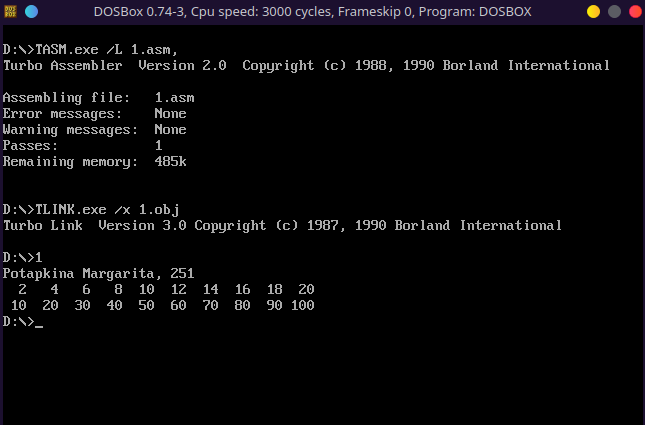
\includegraphics[scale=0.9]{1.png}
\end{figure}

\section{Ответы на контрольные вопросы}
\begin{enumerate}
\item Какой командой можно выделить в памяти место под одномерный массив байтов array размерностью 20?

\begin{minted}{nasm}
array DB 20 DUP (?)
\end{minted}

\item Опишите команды умножения на байт и на слово.

Для умножения беззнаковых чисел используется команда MUL.

Умножение на байт: Один множитель хранится в регистре AL, другой является аргументом команды MUL (например, MUL BL). Результат записывается в AX.

Умножение на слово: Один множитель хранится в регистре AX, другой является аргументом команды MUL (например, MUL BX). Результат записывается в пару регистров DX и AX, причём в DX содержатся старшие 16 бит, а в AX "--- младшие.

\item Какое максимальное беззнаковое число можно хранить в элементе массива размером в 1 байт?

Максимальное беззнаковое число, которое может храниться в элементе массива размером в 1 байт, "--- 255.

\item Пусть имеется массив: array DW 50 DUP(?). Для доступа к отдельным элементам массива используется адресное выражение array[SI]. Как называется этот способ адресации и как с его помощью будет вычисляться адрес элементов массива? 

Такой способ адресации называется индексной со смещением. Адрес элемента массива в таком случае вычисляется путём прибавления к адресу начала массива array относительного адреса (индекса элемента в массиве), записанного в индексном регистре SI.

\item Каким образом осуществляется перебор элементов некоторого массива A с помощью адресного выражения A[SI], если массив состоит из байтов, слов или двойных слов?

Если массив состоит из байтов, то на каждой итерации цикла к SI нужно прибавить 1 (INC SI). Если массив состоит из слов, то SI нужно увеличивать каждый раз на 2 (ADD SI,2). Если из двойных слов "--- то на 4 (ADD SI,4).

\item Для некоторого массива array, объявленного следующим образом: array DW 20 DUP(?), каким будет результат выполнения команды mov DI, array и команды mov DI, offset array?

В первом случае в DI запишется значение первого элемента массива. Во втором же случае будет вычислен адрес начала массива array и уже он будет записан в DI.

\end{enumerate}
% Отобразить все источники. Даже те, на которые нет ссылок.
% \nocite{*}

% Окончание основного документа и начало приложений Каждая последующая секция
% документа будет являться приложением
\appendix
\end{document}
